\chapter{AlterNative}\label{C:AlterNative}
This chapter is a walk-through AlterNative explaining its concept, how it can translate the code, then an example using IOSharp will be used along with some use cases that can be applied to this tool.
\section{Concept}\label{S:AN-Concept}
The concept of AlterNative is to maximize the idea of Internet of Things by providing a tool to port applications from high-level languages (such as .NET) to native languages (such as C++) easily. Most of the actual systems are C++ compatible, thus if the application is ported to this language, it can be executed in several platforms (i.e. smartphones, tablets, embedded systems, computers with different operating systems).
\\
With this tool a developer can take the advantages of fast developing in a high-level languages such as C\# and then gain the advantage of performance related the low-level languages like C++. Apart from this, it also gives the chance to get native code capable of working in several systems, in other words, this philosophy is similar to the WORA (Write Once, Run Anywhere) slogan created by Sun Microsystems to illustrate the cross-platform benefits of Java Virtual Machine. The difference is that AlterNative is focused on the final performance because it outputs the code in native language avoiding the dependence of underlying virtual machines.
\section{Process}\label{S:AN-Process}
AlterNative process is divided in three steps: decompilation, translation and recompilation.
To summarize the following sections the figure \ref{fig:AN-Process} shows the process that is done from the original assembly, the decompilation, translation and finally the recompilation to an another assembly.
\begin{figure}[H]\begin{center}
 \centering
  \captionsetup{justification=centering}
  \includegraphics[width=1\textwidth]{pictures/alternative/process}
  \caption{AlterNative process\label{fig:AN-Process}}
\end{center}\end{figure}

To explain the AlterNative process will be used the \verb!Main! method which both languages make use of it. In the following table is shown how this method looks like in each language.
\begin{table}[htb]
\begin{center}
\begin{tabular}{|c|c|c|}
\hline
{\bf Language} & {\bf Method} & {\bf AST}  \\ \hline \hline
C\#        & \verb!void Main(string[] args){}!    & Figure \ref{fig:AN-AST}       \\ \hline
C++        & \verb!void Main(string args[]){}!    & Figure \ref{fig:AN-AST-Conversions}       \\ \hline
\end{tabular}
\caption{Representation in C\# and C++ of the Main method of a program}
\label{T:AN-Language-Main-Methods}
\end{center}
\end{table}

\subsection{Decompilation}\label{SS:AN-Process-Decom}
First of all the Assembly (compiled program/binary) is passed through a decompiler in order to extract the source code. In this case the original code is in C\# and to decompile it is used a program called ILSpy which is an open-source .NET assembly decompiler. Instead of extracting the code in text format is extracted as an AST (Abstract Syntax Tree) that is an abstract representation with nodes and hierarchies of the original code. This representation is organized in a tree format from the top-level (assembly) until the low-level (instructions, types and constants).
\\
\\
The figure \ref{fig:AN-AST} shows how \verb!void Main(string[] args){}! method would look like in AST format. The top node designates that the child nodes correspond to a method, then in the first row child is described the primitive type (what method returns) which in this case is a \verb!void!, the identifier which shows the method name (\verb!Main!) and finally the parameter declaration which describes the parameters that the function takes. The example method has one parameter corresponding to an array of strings. The parameter declaration node has two nodes defining it, the first one describes that \verb!string[]! is a composed type which is also defined by a string and an array specifier, the second node is the identifier name of the parameter, in this case, \verb!args!.
\begin{figure}[H]\begin{center}
 \centering
  \captionsetup{justification=centering}
  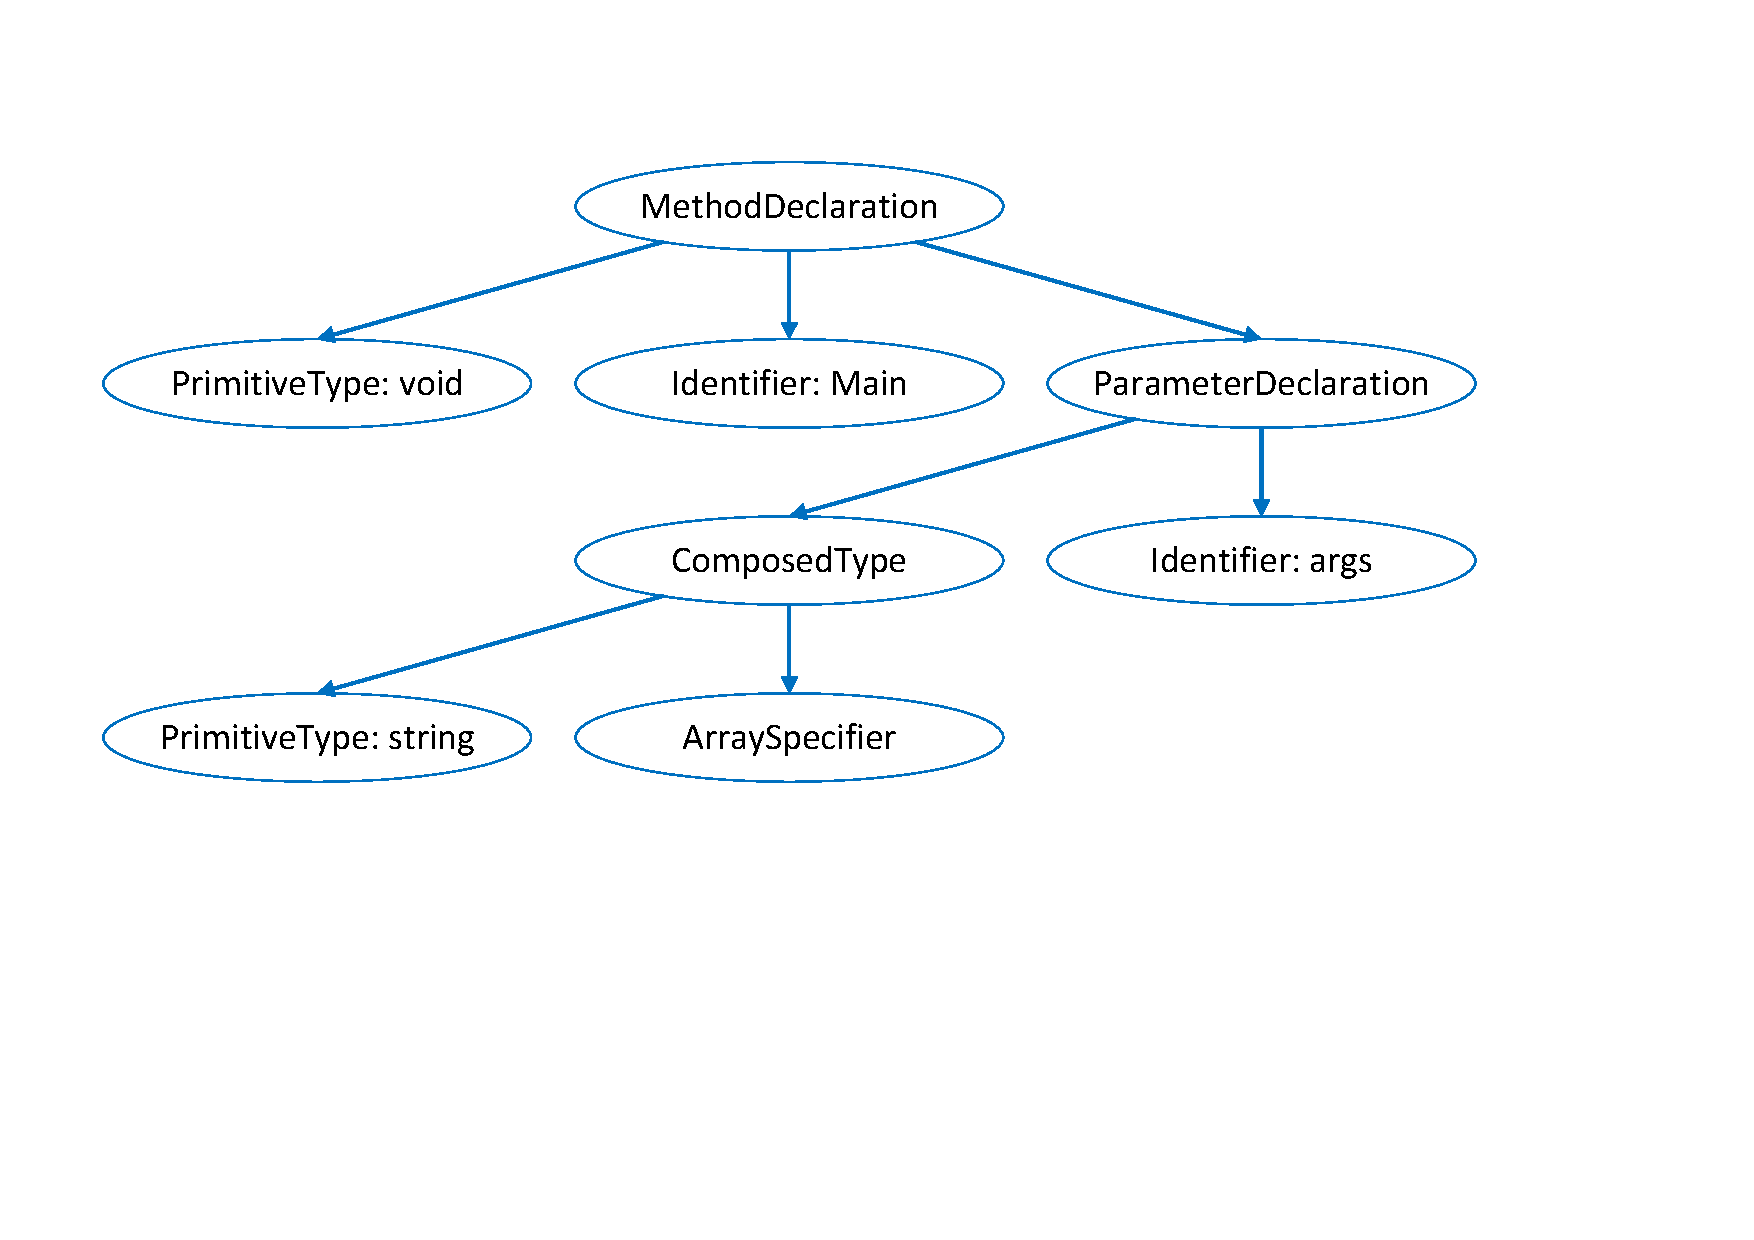
\includegraphics[width=0.7\textwidth]{pictures/alternative/csharp_main_ast}
  \caption{AST representation of the main method in C\#\label{fig:AN-AST}}
\end{center}\end{figure}
The translator will generate the C++ code from the AST representation of the original code.
\subsection{Translation}\label{SS:AN-Process-Translation}
To proceed with the translation is important to know how is the translated language typed, then in order to achieve that some modifications need to be applied to the AST generated in the decompilation time. After doing the pertinent AST modifications a second one will be obtained representing the source code of the desired language. After doing this conversions the following step is start writing the files containing the text representation of the tree. AlterNative translates the code to C++ so the AST changes must be done in a way that the resulting AST corresponds to that language. It is important to remark that C++ is a headed language so headers must be written along with the files containing the code.
\\
\\
Following the example explained in the previous section now the AST will be transformed to the correspond with the C++ one. In C\# the method was \verb!void Main(string[] args){}! but in C++ the syntax is different because the array specifier moves from the primitive type to the identifier. The figure \ref{fig:AN-AST-Conversions} shows in red the changes done to the original tree to achieve an AST corresponding to the C++ method which looks like \verb!void Main(string args[]){}!. The original identifier changes to a composed identifier with two child nodes, the first one is the identifier \verb!args! and the second one is the array specifier which has been moved from the original composed type to the composed identifier in this case. As there is no composed type now the node is deleted and the parameter declaration is directly linked to the primitive type string.
\begin{figure}[H]\begin{center}
 \centering
  \captionsetup{justification=centering}
  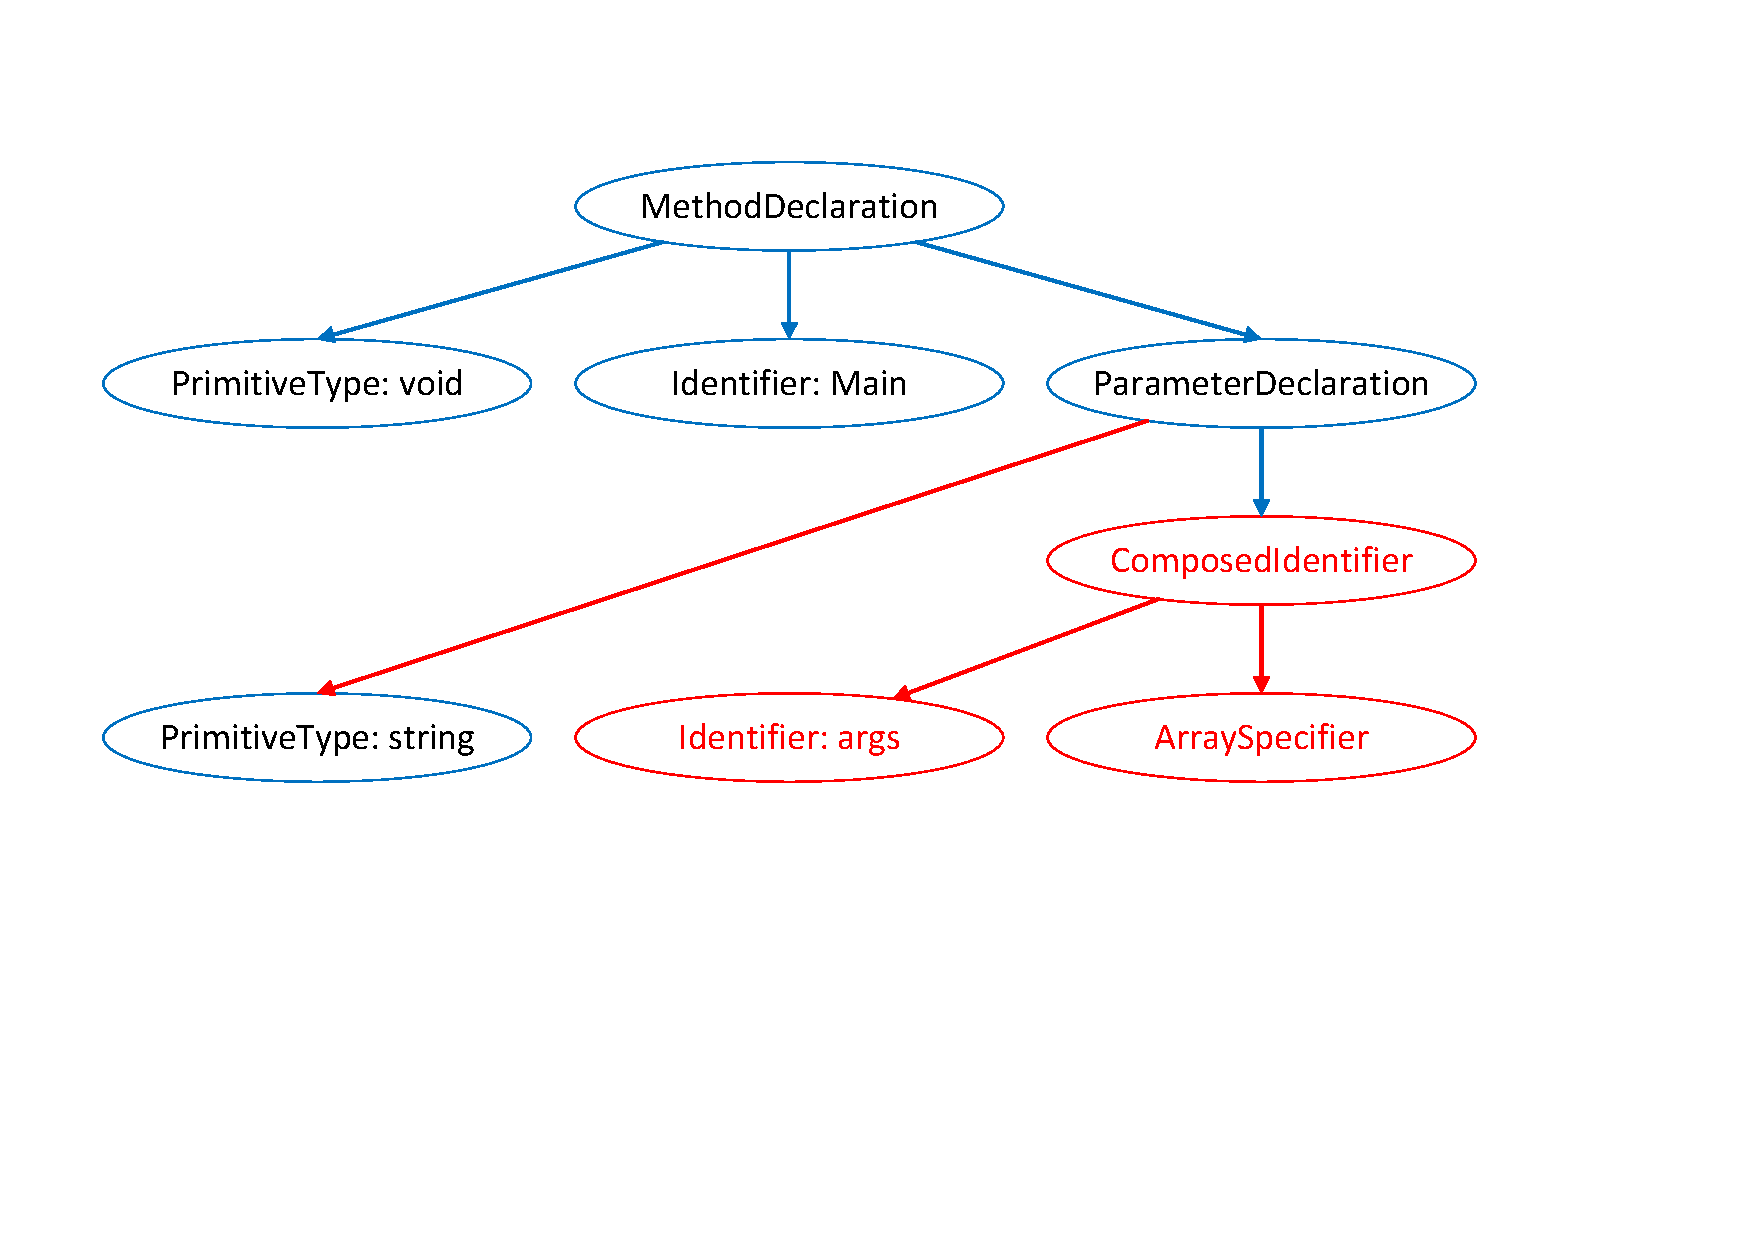
\includegraphics[width=0.7\textwidth]{pictures/alternative/ast_conversions_cpp}
  \caption{AST representation of the main method in C++\label{fig:AN-AST-Conversions}}
\end{center}\end{figure}

\subsection{Recompilation}\label{SS:AN-Process-Recompilation}
The final step consists on compile the C++ code into a new assembly. This final assembly maintains the same functionalities of the first one but taking the benefits of the performance that gives native code. Although it could seem that this software is focused on the code translation it is not its real finality because its aim is to maintain all the features of the original code like the garbage collector, specific expressions or even language syntax. Maintaining this characteristic on mind the programs translated using AlterNative will run much faster than the original because a virtual machine is not required to execute native code.
\\
As mentioned, AlterNative is able to provide most of the features of the original code to the final code using external open-source libraries like the boehm GC for the garbage collector, the boost library for implementing characteristics like threading and delegation and finally a proprietary library which implements all the \verb!System! namespace of C\#. With all of this the final assembly is fully compatible with any system like Windows, Linux, Android or any device capable of execute C++ assemblies.

\section{Use Cases}\label{S:AN-Use-Cases}
There are two clearly use cases of AlterNative together with IOSharp, the first one is performance and the second one is cross-platform for embedded systems.
\subsection{Performance}\label{SS:AN-Use-Cases-Perf}
AlterNative gets the major advantage when is applied to programs or libraries which are very complex in a computational way, for example image processing, mathematics or complex algorithms where languages running on virtual machines are not as fast as the developer needs. The more complex the target is, the more benefit that can be obtained.
Taking into account that the performance seen on IOSharp running on Mono is not as good as it should be compared to the native Micro Framework running on a Netduino. It is supposed that passing a program created with IOSharp through the translator will generate a faster binary because it does not depend on a virtual machine, and it is well known that Mono is not the fastest implementation of the .NET specification.

\subsection{Cross-Platform in embedded systems}\label{SS:AN-Use-Cases-NETMF}
Other advantage of the standard low level languages like C++ is that a high percentage of device processors can execute this code. And at this point is where it fits with the implementation of IOSharp because passing the library through AlterNative a new library will be obtained but instead of being written in C\# it will be in C++. By doing this the generated source can be compiled into an ARM-Linux assembly so the unique requirement to execute that code will be an underlying Linux running on the machine. The developer will get all the benefits of Micro Framework with the speed of C++, the code will be written using the Micro Framework syntax which makes easy the development of embedded applications, and then they could be translated to AlterNative.

\section{Contributions to AlterNative}\label{AN-WorkDone}
To achieve the translation (or partial translation) of IOSharp through AlterNative some work was done on the proprietary implementation of \verb!System! libraries which are the the C++ libraries that externally look like the C\# ones but the methods are implemented using standard C++ functions, the boost libraries or even other libraries like Boehm GC.
\\
\\
At the beginning AlterNative only worked on Windows because some classes from the ILSpy had mixed the view and the decompiler functions so it was unable to run in Linux because the part of the view could not compile. In order to solve that an AlterNative.Core was created which could work in any system that could run C\# code. This core version has its own solution and csproj file but they are pointed to the same code files of the original program. In this way, AlterNative can run either on .NET Framework in Windows or on Mono in Linux and MacOSX.
\\
\\
The first attempt to translate IOSharp was unsuccessful but it helped to determine how near the translation was of being successful. There where several major features that AlterNative was not able to translate like the threading, the delegates used in the interruptions, the P/Invokes or some functions like DateTime, Timer and file reading/writing. Many of those features where required to be implemented on the proprietary library because this is the one that is linked to the translated program in order to run properly.
\\
To implement this features the C++ boost library has been used. This library uses standard C++ functions so it can work practically in any device or operating system. The classes currently implemented either totally or partially are shown in the Appendix \ref{SS:Libs-AlterNative}.
\\
\\
In the figure \ref{fig:AN-Example-IOSharp} is shown the differences between the original Micro Framework, the IOSharp implementation in C\# and the translated one. Each one includes some new layers on the stack either to implement the functionalities of the Micro Framework as IOSharp layer does or to implement the functionalities of C\# like the layer named AlterNative Library which is the implementation of the C\# classes.

\begin{figure}[H]\begin{center}
 \centering
  \captionsetup{justification=centering}
  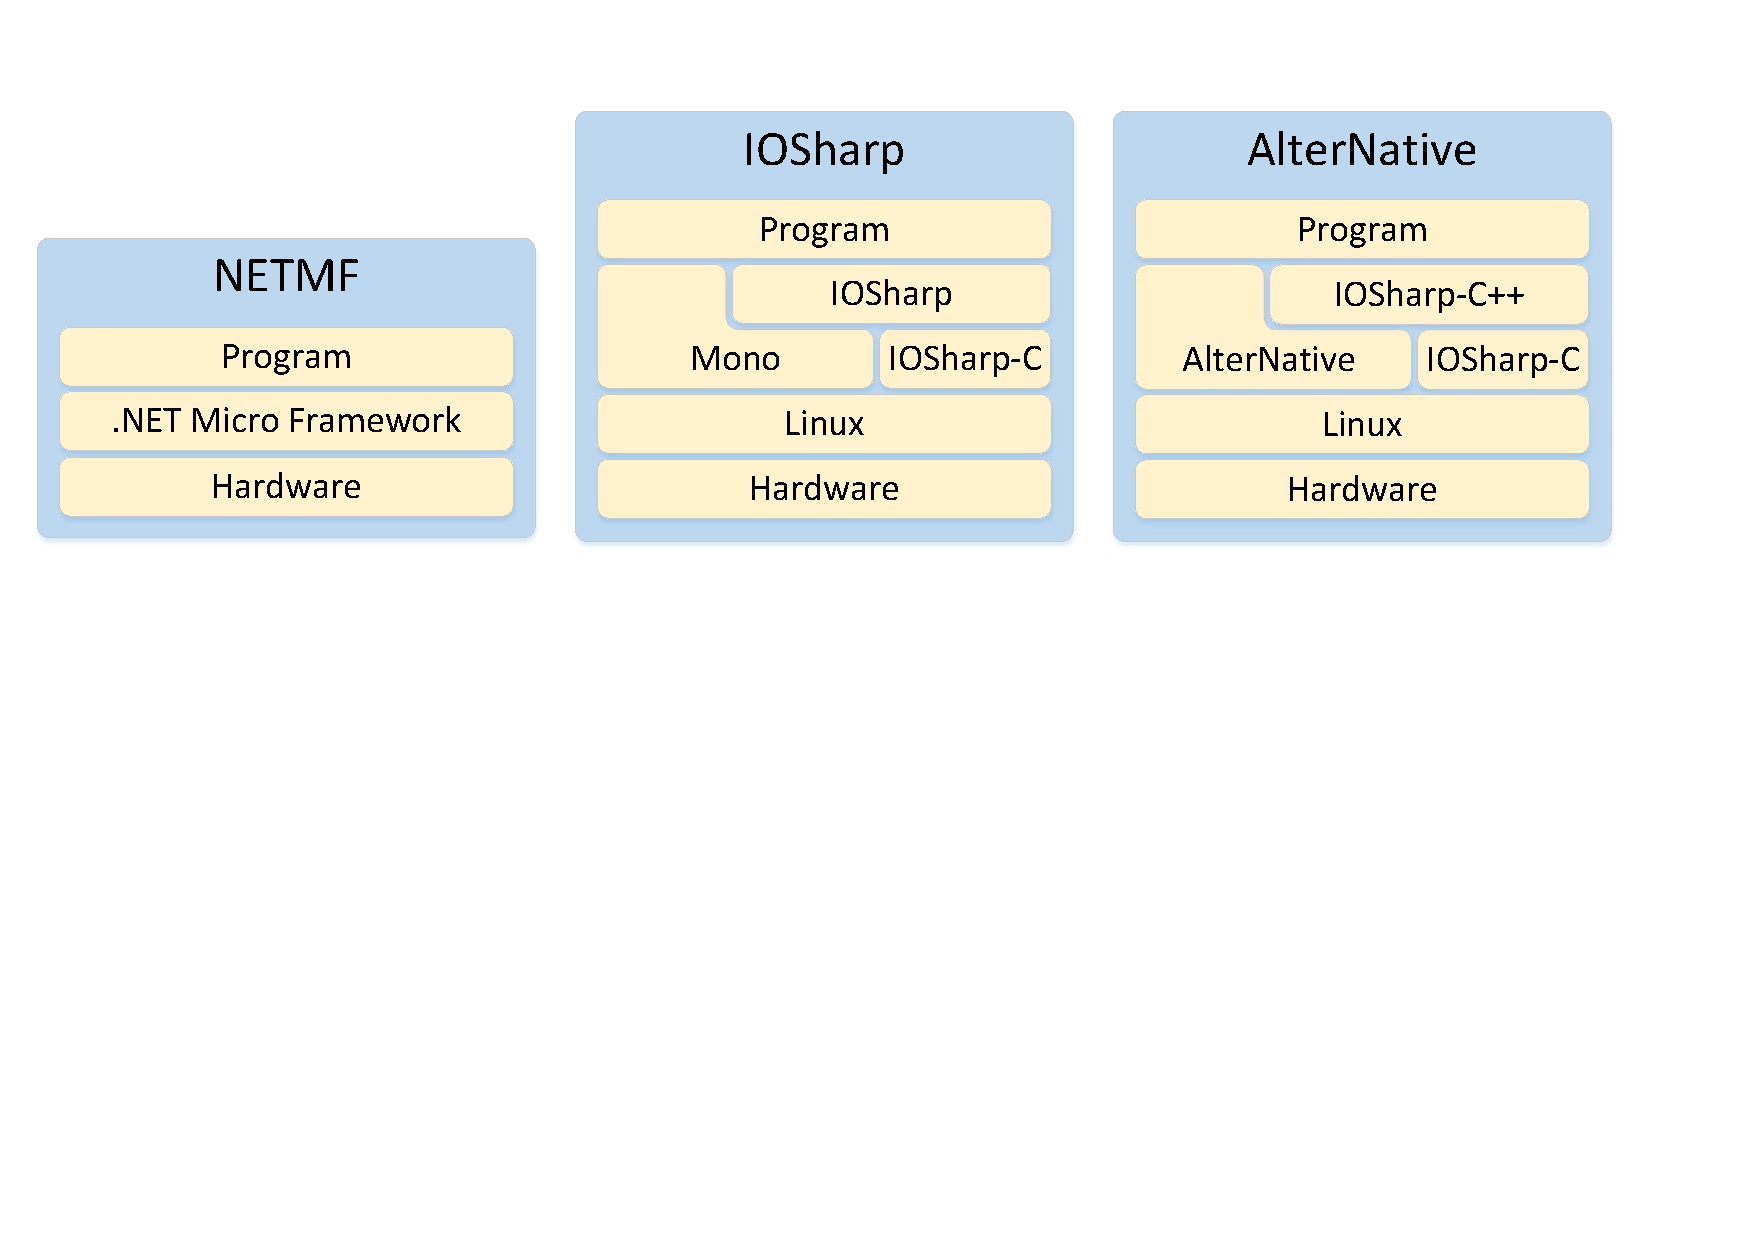
\includegraphics[width=1\textwidth]{pictures/alternative/transformations-iosharp}
  \caption{Stack in the original .NET Micro Framework, the IOSharp implementation and the AlterNative translation\label{fig:AN-Example-IOSharp}}
\end{center}\end{figure}

\section{Example}\label{SS:AN-Process-Example}
The best example to show in this section will be some part of IOSharp translated to C++. In the moment of writing this thesis the only component being 100\% translated automatically was the GPIO ports which basically they use the \gls{SYSFS} of Linux and the interrupt port which uses inter-language calls.

As a short example of this translation the following pieces of code represents the InputPort in the different languages. This first one is the original implementation of IOSharp as it can be downloaded from GitHub.
\begin{lstlisting}[language=CSharp, caption={InputPort in C\#}]
using System;
using System.Collections.Generic;
using System.Linq;
using System.Text;
using Microsoft.SPOT.Hardware;
using IOSharp.NETMF.RaspberryPi.Hardware;
using System.Threading;

namespace raspberrypi
{
    public class InputPort : Port
    {
    	// As it has been explained in the IOSharp seccion, all the GPIO have an inheritance with the Port class, so all of them base to Port.
        public InputPort(Cpu.Pin portId, bool glitchFilter, ResistorMode resistor)
            : base(portId, glitchFilter, resistor, InterruptMode.InterruptNone)
        {
        	// In this case, using the GPIOManager is configured the port as an InputPort
            GPIOManager.Instance.SetPortType(portId, PortType.INPUT);
        }

        protected InputPort(Cpu.Pin portId, bool glitchFilter, ResistorMode resistor, InterruptMode interruptMode)
            : base(portId, glitchFilter, resistor, interruptMode)
        {
            GPIOManager.Instance.SetPortType(portId, PortType.INPUT);
        }

        protected InputPort(Cpu.Pin portId, bool initialState, bool glitchFilter, ResistorMode resistor)
            : base(portId, initialState, glitchFilter, resistor)
        {
            GPIOManager.Instance.SetPortType(portId, PortType.INPUT);
        }

        public ResistorMode Resistor { get; set; }

        public bool GlitchFilter { get; set; }

    }
}
\end{lstlisting}
After translating the project the code is represented in C++ which  uses header files, so the following code represents the header for the InputPort.
\begin{lstlisting}[language=C++, caption={Header file for the InterruptPort in C++}]
#pragma once
#include "System/System.h"
#include "Port.h"
#include "Cpu.h"
#include "GPIOManager.h"
#include "PortType.h"
#include "System/Exception/SystemException/NotImplementedException.h"

using namespace Microsoft::SPOT::Manager;
using namespace System;
namespace Microsoft {
	namespace SPOT {
		namespace Hardware {
			class InputPort : public virtual Port, public virtual Object
			{
				public:
					Port::ResistorMode getResistor();
				public:
					void setResistor(Port::ResistorMode value);
				public:
					bool getGlitchFilter();
				public:
					void setGlitchFilter(bool value);
				public:
					InputPort(Cpu::Pin portId, bool glitchFilter, Port::ResistorMode resistor);
				protected:
					InputPort(Cpu::Pin portId, bool glitchFilter, Port::ResistorMode resistor, Port::InterruptMode interruptMode);
				protected:
					InputPort(Cpu::Pin portId, bool initialState, bool glitchFilter, Port::ResistorMode resistor);
					
				// The C# properties in C++ are automatically converted to variables
				public:
					Port::ResistorMode Resistor_var;
				public:
					bool GlitchFilter_var;
			};
		}
	}
}
\end{lstlisting}
Finally this is the file containing the implementation of the header.
\begin{lstlisting}[language=C++, caption={Implementation of the InterruptPort in C++}]
#include "InputPort.h"
namespace Microsoft {
	namespace SPOT {
		namespace Hardware {
		
			// So the converted variables need to be accessed using getters and setters. Like is shown below
			Port::ResistorMode InputPort::getResistor(){
				return Resistor_var;
			}
			void InputPort::setResistor(Port::ResistorMode value)
			{
				Resistor_var = value;
			}
			bool InputPort::getGlitchFilter()
			{
				return GlitchFilter_var;
			}
			void InputPort::setGlitchFilter(bool value)
			{
				GlitchFilter_var = value;
			}
			InputPort::InputPort(Cpu::Pin portId, bool glitchFilter, Port::ResistorMode resistor) : Port(portId, glitchFilter, resistor, Port::InterruptMode::InterruptNone)
			{
				GlitchFilter_var = (bool)(0);
				Resistor_var = (Port::ResistorMode)(0);
				GPIOManager::getInstance()->SetPortType(portId, PortType::INPUT);
			}
			InputPort::InputPort(Cpu::Pin portId, bool glitchFilter, Port::ResistorMode resistor, Port::InterruptMode interruptMode) : Port(portId, glitchFilter, resistor, interruptMode)
			{
				GPIOManager::getInstance()->SetPortType(portId, PortType::INPUT);
			}
			InputPort::InputPort(Cpu::Pin portId, bool initialState, bool glitchFilter, Port::ResistorMode resistor) : Port(portId, initialState, glitchFilter, resistor)
			{
				throw new NotImplementedException();
			}
		}
	}
}
\end{lstlisting}

Some performance tests had been carried out to quantify how much faster is the translation compared with the original one running on Mono. The explanation of the tests and its results are on the next chapter.